\newcommand*{\VorlagenPfad}{../../../../Vorlagen}%
\documentclass{\VorlagenPfad/coderdojokabeamer}

\title{Bedingungen und Falls-Abfragen}
\author{CoderDojo Karlsruhe}
\date{April 24, 2015}

\begin{document}

\maketitle

\section{Bedingungen}

\begin{frame}{Bedingungen}
  "Wenn morgen die Sonne scheint, gehe ich ins Schwimmbad"
\end{frame}

\begin{frame}{Falls-Abfrage}
	Falls \textless scheint morgen die Sonne?\textgreater:\\
	\noindent\hspace*{12mm} gehe\_ins\_Schwimmbad()
\end{frame}

\begin{frame}{Bedingungen}
	Eine Bedingung ist eine Aussage, die nur zu Ja(Wahr) oder Nein(Falsch) ausgewertet werden kann.
\end{frame}

\begin{frame}{Bedingungen mit Alternativen}
	"Wenn morgen die Sonne scheint, gehe ich ins Schwimmbad, ansonsten ins Kino"
\end{frame}

\begin{frame}{Falls-Ansonsten-Abfrage}
	Falls \textless scheint morgen die Sonne?\textgreater:\\
	\noindent\hspace*{12mm} gehe\_ins\_Schwimmbad()\\
	Ansonsten:\\
	\noindent\hspace*{12mm} gehe\_ins\_Kino()
\end{frame}

\section{Bedingungen verknüpfen}

\begin{frame}{Bedingungen verknüpfen mit Und}
	Wenn morgen die Sonne scheint UND es wärmer als $25^{\circ}C$ ist, gehe ich ins Schwimmbad.
 \begin{table}[t,clr]
 	\begin{center}
 		\begin{tabular}{|l|l|l|l|}
 			\hline
 			Sonne scheint	& wärmer als $25^{\circ}$	& Ergebnis	\\ \hline\hline
 			wahr			& falsch					&			\\ \hline
 			wahr			& wahr						&			\\ \hline
 			falsch			& falsch					&			\\ \hline
 			falsch			& wahr						&			\\ \hline
 		\end{tabular}
 	\end{center}
 \end{table}
\end{frame}

\begin{frame}{Bedingungen verknüpfen mit Oder}
	Wenn morgen die Sonne scheint ODER es wärmer als $25^{\circ}C$ ist, gehe ich ins Schwimmbad.
	\begin{table}[t,clr]
		\begin{center}
			\begin{tabular}{|l|l|l|l|}
				\hline
				Sonne scheint	& wärmer als $25^{\circ}$	& Ergebnis	\\ \hline\hline
				wahr			& falsch					&			\\ \hline
				wahr			& wahr						&			\\ \hline
				falsch			& falsch					&			\\ \hline
				falsch			& wahr						&			\\ \hline
			\end{tabular}
		\end{center}
	\end{table}
\end{frame}

\section{Im Code}

\begin{frame}{Scratch}
  \begin{figure}[t]
    \centering
    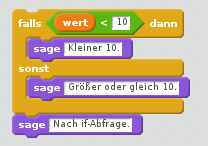
\includegraphics[scale=.6]{scratch_if_else}
    \caption{Falls-Ansonsten in Scratch}
  \end{figure}
\end{frame}

\begin{frame}[fragile]{Python}
  \begin{minted}{python}
  if wert < 10:
      print("Kleiner 10.")
  else:
      print("Größer oder gleich 10.")

  print("Nach if-Abfrage.")
  \end{minted}
\end{frame}

\end{document}
